\documentclass[twocolumn,a4paper]{article}
\usepackage{graphicx}
\usepackage{amsfonts}
\usepackage{color}
\usepackage{lineno}
\setlength{\columnsep}{10pt}
\setlength{\oddsidemargin}{0pt}
\setlength{\topmargin}{0pt}
\setlength{\headheight}{0pt}
\setlength{\headsep}{0pt}
\setlength{\marginparsep}{0pt}
\setlength{\marginparwidth}{0pt}
\addtolength{\voffset}{-50pt}
\setlength{\textheight}{26.8cm}
\author{Siwang Li}

\title{Elastic Material Optimization}

%% document begin here
\begin{document}
\maketitle

\section{Summary}


\section{Input} 
In the following experiment, we use an implicit integrator instead of an
harmonic oscillator to produce the input animations.

\section{Experiments}
In the first experiment, we check the numerical damping of the implicit
integrated result of one mode, with
$\lambda=0.5,\alpha_k=\alpha_m=0,T=500$. Then,we optimize for both $k$ and
$d$. The residuals are $|k-\lambda|=0$, $E(k,d)=1\times 10^{-27}$, and the
optimized damping is $d=0.05$. We draw the input sequence $z_1,\cdots,z_T$, and
the curve of $z(k,d)$(using the harmonic oscillator) in figure
\ref{onemode}. They are overlapped.
\begin{figure}
  \centering
  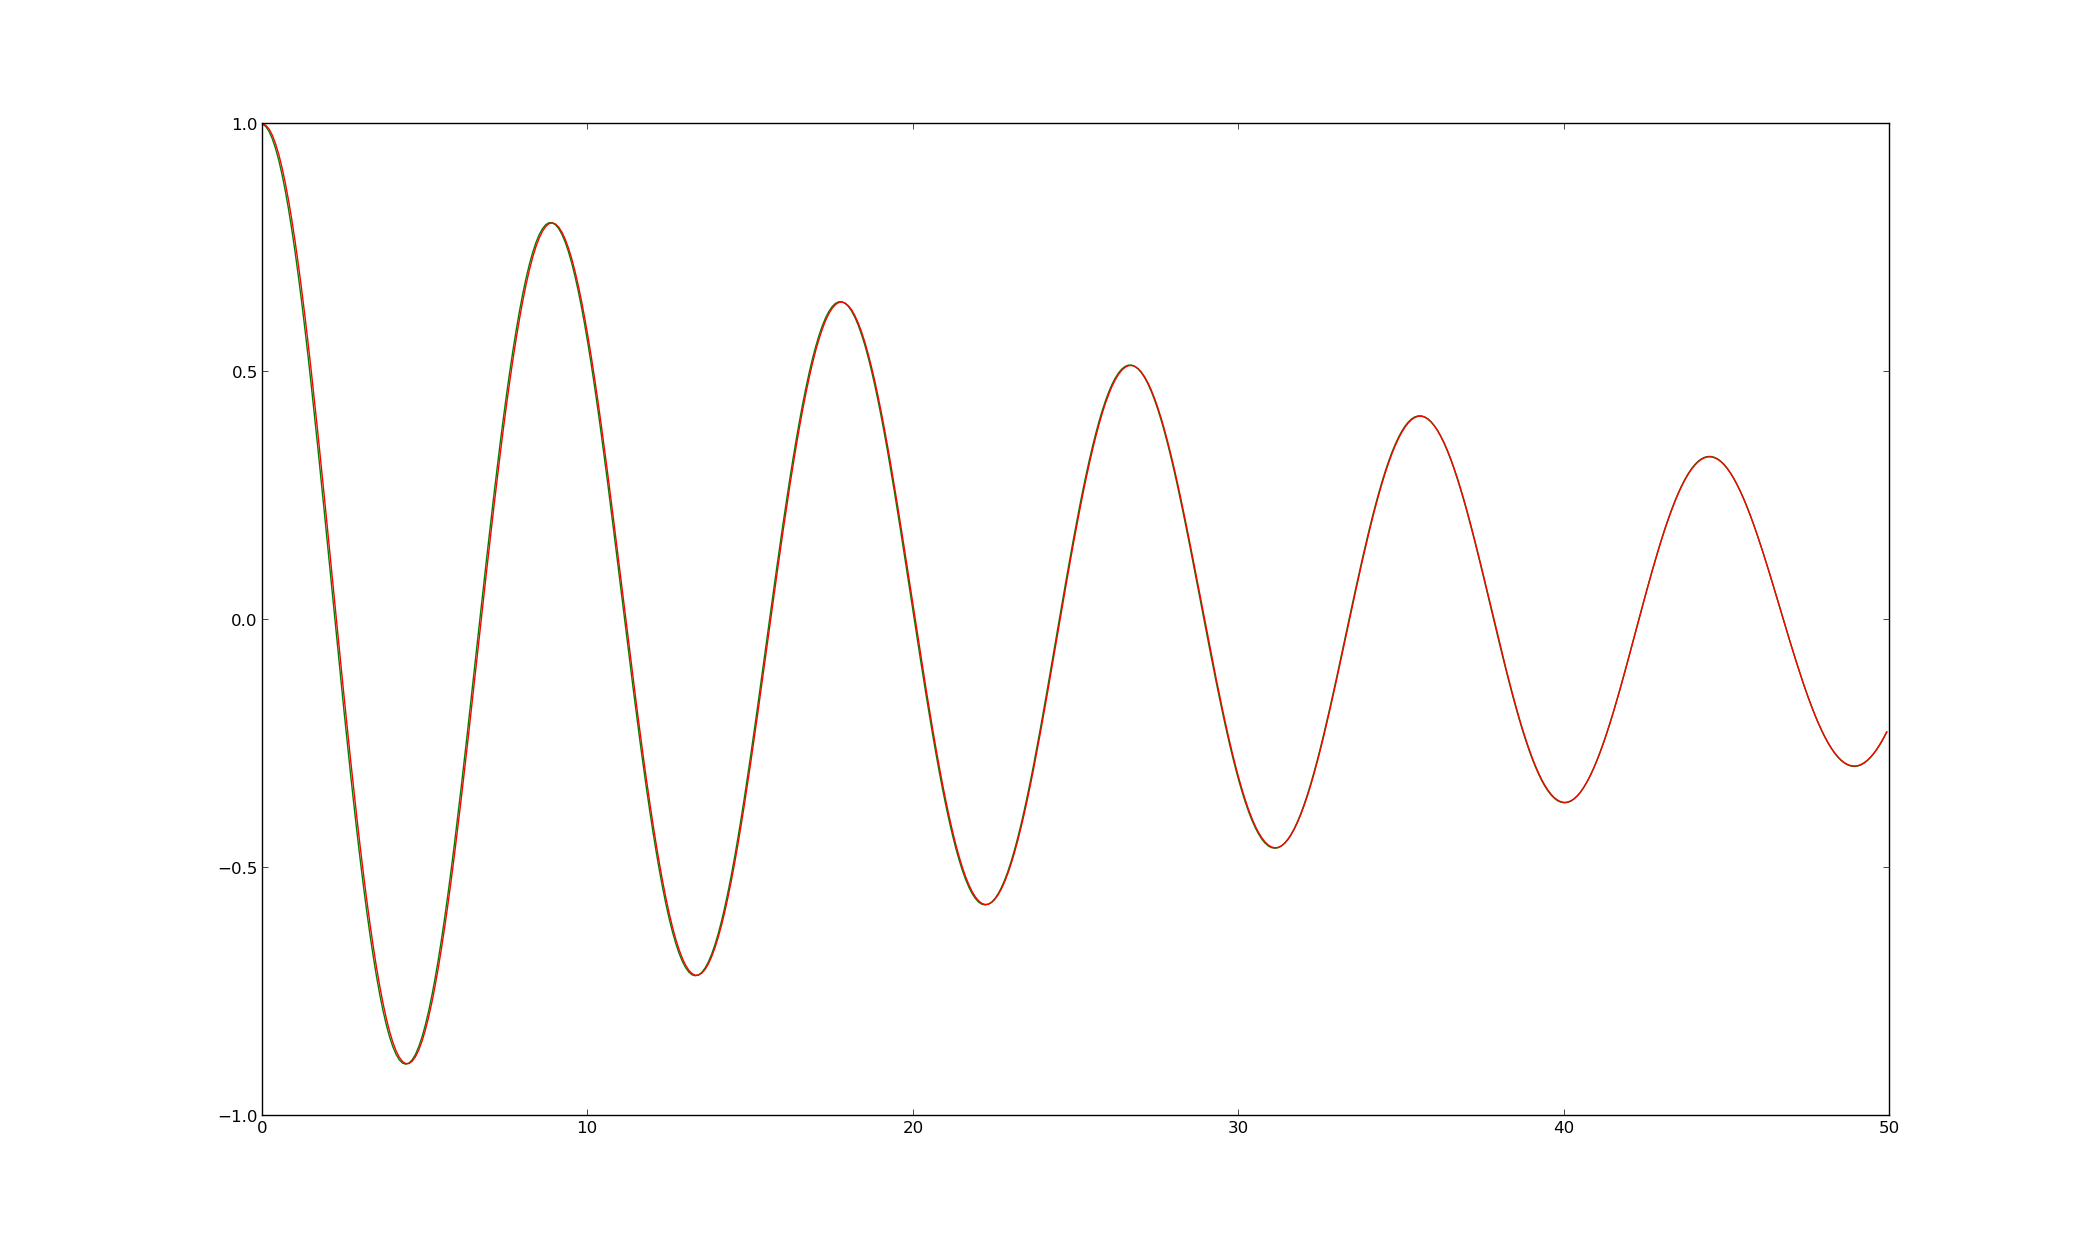
\includegraphics[width=0.48\textwidth]{figures/singleModeDK_imp.png}
  \caption{Green is input and red is output. They are overlapped.}
  \label{onemode}
\end{figure}

In the second experiment, we use $5$ modes to produce the input animation. And
then we optimize for $D(d)=diag(d_1,\cdots,d_5)$, and $K(k)$(dense,
symmetric). The resulting $K$ is very close to a diagonal matrix(the off
diagonal elements are less than $10^{-11}$), and the elements in the diagonal
are equal to the eigenvalues that are used to produce the input animation.

In the third experiment, we check the whole approximation residuals with an
animation sequence in full space as input. We produce this sequence using a RS
simulator, without constraints or external forces.

The fourth experiment is similar to the above one, except that we produce the
input animation using a full StVK simulator.

After making the above experiments, we can begin to check the impact of the
external forces and constraints. And firstly, we check impact of the external
forces, and we also start from a single mode.

\end{document}